\documentclass{sigchi}

% Use this command to override the default ACM copyright statement
% (e.g. for preprints).  Consult the conference website for the
% camera-ready copyright statement.

%% EXAMPLE BEGIN -- HOW TO OVERRIDE THE DEFAULT COPYRIGHT STRIP -- (July 22, 2013 - Paul Baumann)
% \toappear{Permission to make digital or hard copies of all or part of this work for personal or classroom use is      granted without fee provided that copies are not made or distributed for profit or commercial advantage and that copies bear this notice and the full citation on the first page. Copyrights for components of this work owned by others than ACM must be honored. Abstracting with credit is permitted. To copy otherwise, or republish, to post on servers or to redistribute to lists, requires prior specific permission and/or a fee. Request permissions from permissions@acm.org. \\
% {\emph{CHI'14}}, April 26--May 1, 2014, Toronto, Canada. \\
% Copyright \copyright~2014 ACM ISBN/14/04...\$15.00. \\
% DOI string from ACM form confirmation}
%% EXAMPLE END -- HOW TO OVERRIDE THE DEFAULT COPYRIGHT STRIP -- (July 22, 2013 - Paul Baumann)

% Arabic page numbers for submission.  Remove this line to eliminate
% page numbers for the camera ready copy
% \pagenumbering{arabic}

% Load basic packages
\usepackage{balance}  % to better equalize the last page
\usepackage{graphics} % for EPS, load graphicx instead 
\usepackage[T1]{fontenc}
\usepackage{txfonts}
\usepackage{mathptmx}
\usepackage[pdftex]{hyperref}
\usepackage{color}
\usepackage{booktabs}
\usepackage{textcomp}
% Some optional stuff you might like/need.
\usepackage{microtype} % Improved Tracking and Kerning
% \usepackage[all]{hypcap}  % Fixes bug in hyperref caption linking
\usepackage{ccicons}  % Cite your images correctly!
% \usepackage[utf8]{inputenc} % for a UTF8 editor only

\usepackage{chemformula}
\usepackage{booktabs,amsmath}
\usepackage[utf8]{inputenc}
\usepackage{array}
\usepackage{multirow}
\usepackage{graphicx}
\usepackage{wrapfig}
\usepackage{placeins}
\usepackage{float}
\usepackage{amssymb}
\usepackage{pdfpages}
\usepackage{chemformula}
\usepackage{amsmath}
\usepackage{caption}
\usepackage{subcaption}
%\usepackage{subfig}

% If you want to use todo notes, marginpars etc. during creation of your draft document, you
% have to enable the "chi_draft" option for the document class. To do this, change the very first
% line to: "\documentclass[chi_draft]{sigchi}". You can then place todo notes by using the "\todo{...}"
% command. Make sure to disable the draft option again before submitting your final document.
\usepackage{todonotes}

% Paper metadata (use plain text, for PDF inclusion and later
% re-using, if desired).  Use \emtpyauthor when submitting for review
% so you remain anonymous.
\def\plaintitle{SIGCHI Conference Proceedings Format}
\def\plainauthor{First Author, Second Author, Third Author,
  Fourth Author, Fifth Author, Sixth Author}
\def\emptyauthor{}
\def\plainkeywords{Authors' choice; of terms; separated; by
  semicolons; include commas, within terms only; required.}
\def\plaingeneralterms{Documentation, Standardization}

% llt: Define a global style for URLs, rather that the default one
\makeatletter
\def\url@leostyle{%
  \@ifundefined{selectfont}{
    \def\UrlFont{\sf}
  }{
    \def\UrlFont{\small\bf\ttfamily}
  }}
\makeatother
\urlstyle{leo}

% To make various LaTeX processors do the right thing with page size.
\def\pprw{8.5in}
\def\pprh{11in}
\special{papersize=\pprw,\pprh}
\setlength{\paperwidth}{\pprw}
\setlength{\paperheight}{\pprh}
\setlength{\pdfpagewidth}{\pprw}
\setlength{\pdfpageheight}{\pprh}

% Make sure hyperref comes last of your loaded packages, to give it a
% fighting chance of not being over-written, since its job is to
% redefine many LaTeX commands.
\definecolor{linkColor}{RGB}{6,125,233}
\hypersetup{%
  pdftitle={\plaintitle},
% Use \plainauthor for final version.
%  pdfauthor={\plainauthor},
  pdfauthor={\emptyauthor},
  pdfkeywords={\plainkeywords},
  bookmarksnumbered,
  pdfstartview={FitH},
  colorlinks,
  citecolor=black,
  filecolor=black,
  linkcolor=black,
  urlcolor=linkColor,
  breaklinks=true,
}

% create a shortcut to typeset table headings
% \newcommand\tabhead[1]{\small\textbf{#1}}

% End of preamble. Here it comes the document.
\begin{document}

\title{Project Report: Finite Element Analysis for OsteoApp}

\numberofauthors{3}
\author{%
  \alignauthor{Baihan Lin\\
    \affaddr{UbiComp Lab}\\
    \affaddr{University of Washington}\\
    \affaddr{Seattle, WA 98105, USA}\\
    \email{doerlbh@gmail.com}}\\
}

\maketitle

\begin{abstract}
The project aims to conduct a finite element analysis (FEA) on a bone-like structure to simulate the vibration properties of a bone or arm. This simulation is supportive to OsteoApp, a smartphone app for personal osteoporosis screening that tests bone density and tells people if they are at risk for bone disease. OsteoApp uses a vibration technique that takes advantage of the accelerometers on a hand-held smartphone to measure bone stiffness and density, based on the vibrations that pass through the user's arm when the elbow is tapped. The FEA simulation in this study can help us better understand the relationship between the external tapping with the measured signals. This study is conducted by Baihan Lin, mentored by Morelle Arian and Josh Fromm, and supervised by Prof. Shwetak Patel.

\end{abstract}

\category{H.5.m.}{Information Interfaces and Presentation
 (e.g. HCI)}{Miscellaneous}{}{}

\keywords{signal processing, ubiquitous computing, health sensing, mobile phones, osteoporosis screening, finite elements analysis}

\section{Introduction}

Osteoporosis is a disease where increased bone weakness increases the risk of a broken bone. OsteoApp aims to utilize the accelerometers on a hand-held smartphone to measure bone strength, based on the vibrations that pass through the user's arm when the elbow is tapped. To facilitate the understanding of the relationship between the external tapping with the measured signals, finite element analysis (FEA) is applied, as a computerized method for predicting how a product reacts to real-world forces, vibration, heat, fluid flow, and other physical effects. The study aims to understand the information that accelerometers may be collecting based on the simulated properties of the bone-like structures. \\

The study plans for three stages:
\begin{itemize}
\item simulate a simplified bone-like structure
\item simulate the bone with more details and less assumptions
\item formulate the equations of the signal properties
\newline
\end{itemize}

For each bone models, several FEA analyses can be conducted:
\begin{itemize}
\item static stress analysis
\item natural frequency analysis
\item drop test analysis with rigid impact
\item drop test analysis with flexible impact
\item drop test analysis with damping effect
\item linear dynamic modeling with modal damping 
\end{itemize}

\section{Progress} 

UPDATE-\today: Currently, I have conducted multiple simulations for a simplified combined model of bones (a wooden complex combining two bent rods). I also created the basic formula of the natural frequency of the bone.

\subsection{2017/03/30: Interview and Setup}

Morelle warmly introduced me to the project and we briefly discussed the general idea of the OsteoApp project as well as its current state. 

\subsection{2017/04/04: Decide on project}

Josh, Morelle and I discussed about the two directions of the supporting simulation analysis for OsteoApp. We decided that there are two major directions: one is to simulate the entire finite element analysis in SolidWorks; the other is to biophysically define and formulate the possible equations of bone vibration based on the limited physical properties of bone structures. 
After some discussion, we finally decided to start from SolidWorks simulations and later march towards mathematical formulation which is more creative and challenging.

\subsection{2017/04/11: Basic construction of model}

As shown in Figure~\ref{fig:arm_diagram} from $Grey's$ $Anatomy$ \cite{WikipediaEN:Arm}, the humerus is the (upper) arm bone which joins with the scapula above at the shoulder joint (or glenohumeral joint) and with the ulna and radius below at the elbow joint. The entire structure of bones is rather complicated considering the twisted and combined configuration.


\begin{figure}
\centering
  \includegraphics[width=0.9\columnwidth]{figures/human_arm_bones_diagram}
  \caption{Bones of the upper limbs, together with shoulder girdles together comprising the human arm}~\label{fig:arm_diagram}
\end{figure}


To simplify the arm structure, I first use femur bone model from GrabCAD \cite{SB:bone} for my initial simulation, with its shape shown and its mass properties shown in Figure \ref{fig:femur_property}. However, later I found that the calculation by SolidWorks took several hours for even the simplest simulation. I attributed this issue as the complexity of the real bone structure as well as its fine mesh mapping. 


\begin{figure}
\centering
  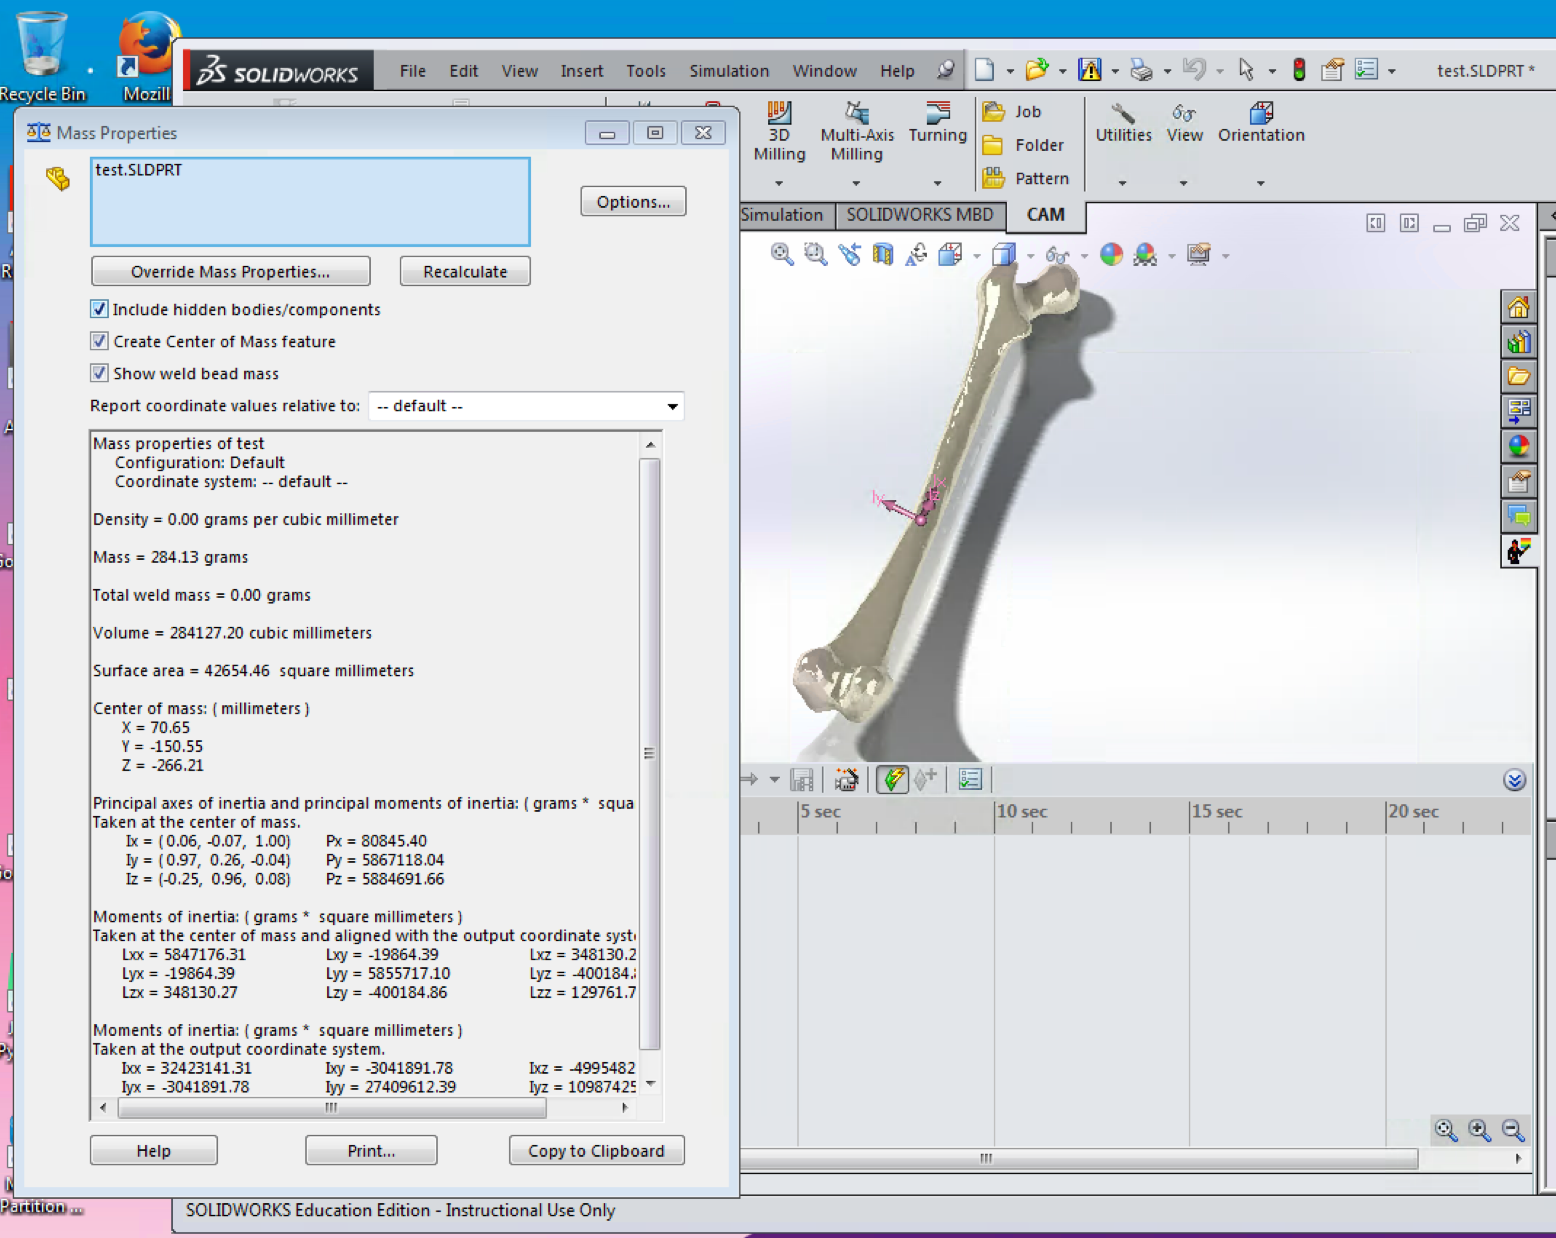
\includegraphics[width=0.9\columnwidth]{figures/femur_property}
  \caption{the femur model and its mass properties }~\label{fig:femur_property}
\end{figure}


Therefore, I created a 3D model of a simplified double bone of ulna and radius combined, shown in Figure \ref{fig:double_bone}. To create the bone, I assume an average adult has ulna and radius bone with an approximately 20mm in diameter each and 300mm in length with a flex of 15 degrees. I combined them together with a shared diameters of 2mm from the flex. 


\begin{figure}
\centering
  \includegraphics[width=0.9\columnwidth]{figures/double_bone}
  \caption{the double bone model}~\label{fig:double_bone}
\end{figure}


For the material selection applied for simulations, the bones are not fully solid but made up of a network of matter with pores. In addition, most of the largest bones are hollow and each bone also contains blood vessels, nerve cells and living bone cells known as osteocytes. These are held together by a framework of hard, non-living material containing calcium and phosphorous. A thin membrane called the periosteum covers the surface of your bones. Based on different density, bone can either be spongy or compact. Therefore, I suppose the nearest to bone would be a composite of some sort or hard-wood, because trunks also consist of cells with cell walls like bone structures. From the material categories, I chose balsa wood as the structure with properties shown in Figure \ref{fig:db_balsa}.

\begin{figure}
\centering
  \includegraphics[width=0.9\columnwidth]{figures/db_balsa}
  \caption{the material properties of balsa wood applied to the designed double bone model}~\label{fig:db_balsa}
\end{figure}

\subsubsection{Static stress analysis}

With a fixed point on the top of the bone as a hand holding smartphone, the simulation exert a static 20N force in a direction normal to the bottom of the combined double bone model, resembling the movement of tapping the elbow.

The static stress analysis doesn't inform much about frequency signals. However, as shown in Figure \ref{fig:db_stat_ana}, it offers helps information on the biggest strain of the model, which can also be the noisiest location to collect signals. This can possibly imply the evaluation of signal qualities based on certain posture of holding the phone.


\begin{figure*}
\centering
  \includegraphics[width=1.95\columnwidth]{figures/db_stat_ana}
  \caption{the static stress analysis of the double bone model in (a) stress, (b) displacement and (c) strain.}~\label{fig:db_stat_ana}
\end{figure*}


\subsubsection{Natural frequency analysis}

Natural Frequencies are the fundamental frequencies whose multiples are called "harmonics". The model structures tend to vibrate with a particular mode shape at each frequency. Dynamic loads coinciding with a natural frequency can cause resonance. Therefore, we can measure its natural frequency as a potential signal indicator via resonance. Damping exists in real structures to limit the response.

It is also noted that, natural frequencies and mode shapes depend on geometry, material properties and mass, support conditions (fixtures) and in-plane loads. Many of these factors have been simplified by assumptions which can be different from a real bone structures. Thus, further study can be conducted to explore these factors. In addition, real structures have infinite numbers of natural frequencies and modal shapes, but in finite element models we use, they only have a finite number.

The simulation indicates a wide variety of possible harmonic vibrations, as shown from Figure \ref{fig:db_freq1}. The relationship of mode number with natural frequencies were not purely linear, demonstrated by Table \ref{tab:db_freq} and Figure \ref{fig:db_freq1_graph1}.

\begin{figure*}
  \centering
  \includegraphics[width=1.95\columnwidth]{figures/db_freq1}
  \caption{natural frequency analysis for double bone}
    ~\label{fig:db_freq1}
\end{figure*}

\begin{table}
  \centering
  \begin{tabular}{l r r r}
    % \toprule
    & & \multicolumn{2}{c}{\small{\textbf{Frequency}}} \\
    \cmidrule(r){3-4}
    {\small\textit{Mode No.}}
    & {\small \textit{Period (s)}}
      & {\small \textit{(Rad/s)}}
    & {\small \textit{(Hertz)}} \\
    \midrule
    1 & 0.0076324 & 823.23 & 131.02 \\
    2 & 0.0051459 & 1221 & 194.33 \\
    3 & 0.0014234 & 4414.1 & 702.53 \\
    4 & 0.0012319 & 5100.4 & 811.76 \\
    4 & 0.0011668 & 5384.9 & 857.04 \\
    % \bottomrule
  \end{tabular}
  \caption{natural frequencies in different modes for double bone model}~\label{tab:db_freq}
\end{table}

\begin{figure}
\centering
  \includegraphics[width=0.9\columnwidth]{figures/db_freq1_graph1}
  \caption{natural frequency vs. mode number for double bone}~\label{fig:db_freq1_graph1}
\end{figure}


\subsubsection{Drop test analysis with rigid impact}

In a drop test analysis, the time varying stresses and deformations due to an initial impact of the product with a rigid or flexible planar surface (the floor) are calculated. I found this simulation interesting because the idea of tapping elbow resembles dropping the elbow on a desk or hand. 

I found another variable very useful that is generated in the analysis, "Translational Acceleration" in $mm/s^2$, because I think this signal could potentially resemble the signal sensed by the accelerometers in smartphones.

In Drop Test 1, the bone vertically drop at 5m/s with gravity considered. In this case, I consider the system without damping, so I set contact damping = 0. I also consider it to drop to a stiff surface, so I set target stiffness = rigid, with result shown in Figure \ref{fig:db_dt1_ana}. 

Interestingly, if we consider the time graph of the translational acceleration (Figure \ref{fig:db_dt1_res}) as described previously, we can see that the signals have their unique patterns. Node 1 and 2 were both collected at the very end, and they responded different from Node 7 in a more middle position.

\begin{figure*}
  \centering
  \includegraphics[width=1.95\columnwidth]{figures/db_dt1_ana}
  \caption{analysis for Drop Test 1 for double bone in (a) stress, (b) displacement and (c) strain.}
    ~\label{fig:db_dt1_ana}
\end{figure*}

\begin{figure*}
  \centering
  \includegraphics[width=1.95\columnwidth]{figures/db_dt1_res}
  \caption{response graphs for Drop Test 1 for double bone in three different location (nodes).}
    ~\label{fig:db_dt1_res}
\end{figure*}

\subsubsection{Drop test analysis with flexible impact}

In Drop Test 2, the bone vertically drop at 5m/s with gravity considered. In this case, I consider the system without damping, so I set contact damping = 0. I also consider it to drop to a flexible surface, so I set target stiffness = flexible, with result shown in Figure \ref{fig:db_dt2_ana}. 

I found this case interesting because this resembles the tapping of elbow by hand palm which is a flexible surface with certain thickness. From the animation I also observe such absorption of vibrations and delay of transduction.

If we consider the time graph of the translational acceleration (Figure \ref{fig:db_dt2_res}), we can see that the signals are in fact very different from the Drop Test 1 in the same locations. This implies that the material of the tapping objects is a very important factor in the signal identification.

\begin{figure*}
  \centering
  \includegraphics[width=1.95\columnwidth]{figures/db_dt2_ana}
  \caption{analysis for Drop Test 2 for double bone in (a) stress, (b) displacement and (c) strain.}
    ~\label{fig:db_dt2_ana}
\end{figure*}

\begin{figure*}
  \centering
  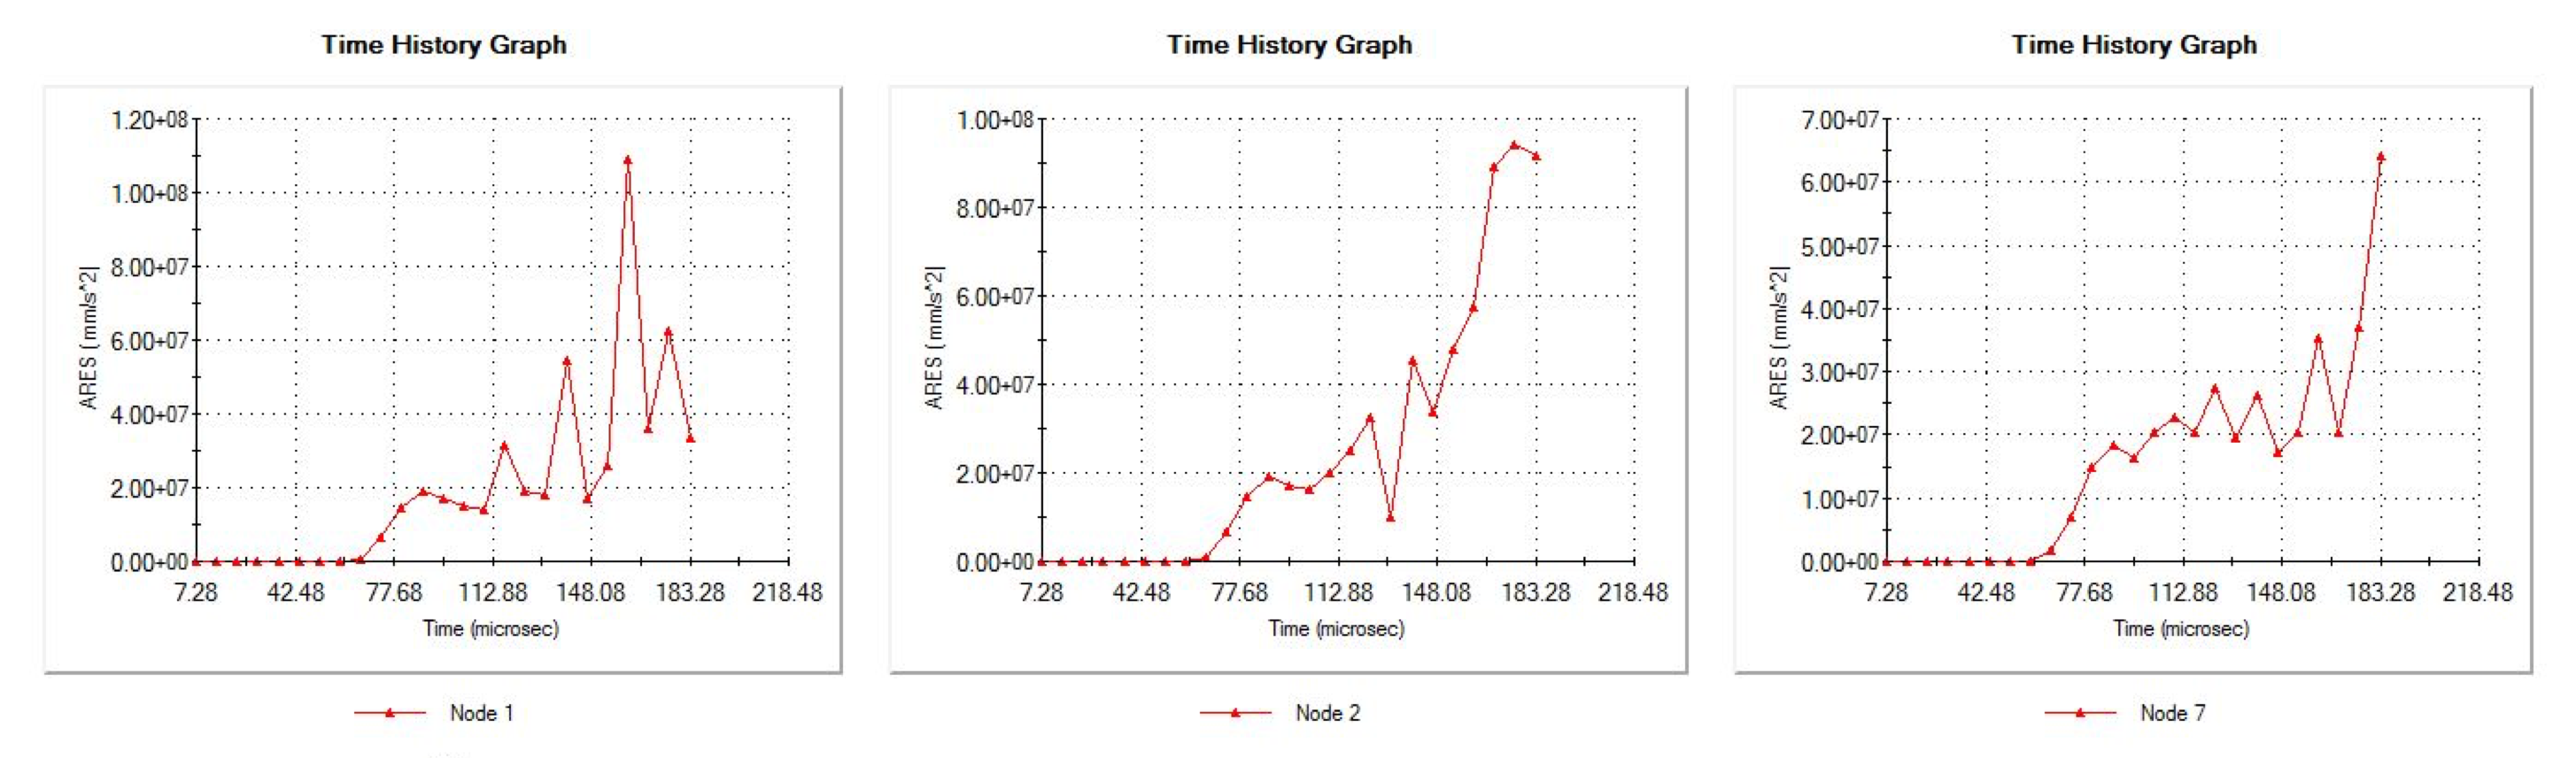
\includegraphics[width=1.95\columnwidth]{figures/db_dt2_res}
  \caption{response graphs for Drop Test 2 for double bone in three different location (nodes).}
    ~\label{fig:db_dt2_res}
\end{figure*}


\subsubsection{Drop test analysis with damping effect}

In Drop Test 3, the bone vertically drop at 5m/s with gravity considered. In this case, I consider the system without damping, so I set contact damping = 0.5. I also consider it to drop to a stiff surface, so I set target stiffness = rigid, with result shown in Figure \ref{fig:db_dt3_ana}, which is very similar to Drop Test 1. Such similarity also arises in the time graph of the translational acceleration (Figure \ref{fig:db_dt3_res}). Arguably speaking, this doesn't support the importance of damping effect in signal feature extraction later in OsteoApp development. 

\begin{figure*}
  \centering
  \includegraphics[width=1.95\columnwidth]{figures/db_dt3_ana}
  \caption{analysis for Drop Test 3 for double bone in (a) stress, (b) displacement and (c) strain.}
    ~\label{fig:db_dt3_ana}
\end{figure*}

\begin{figure*}
  \centering
  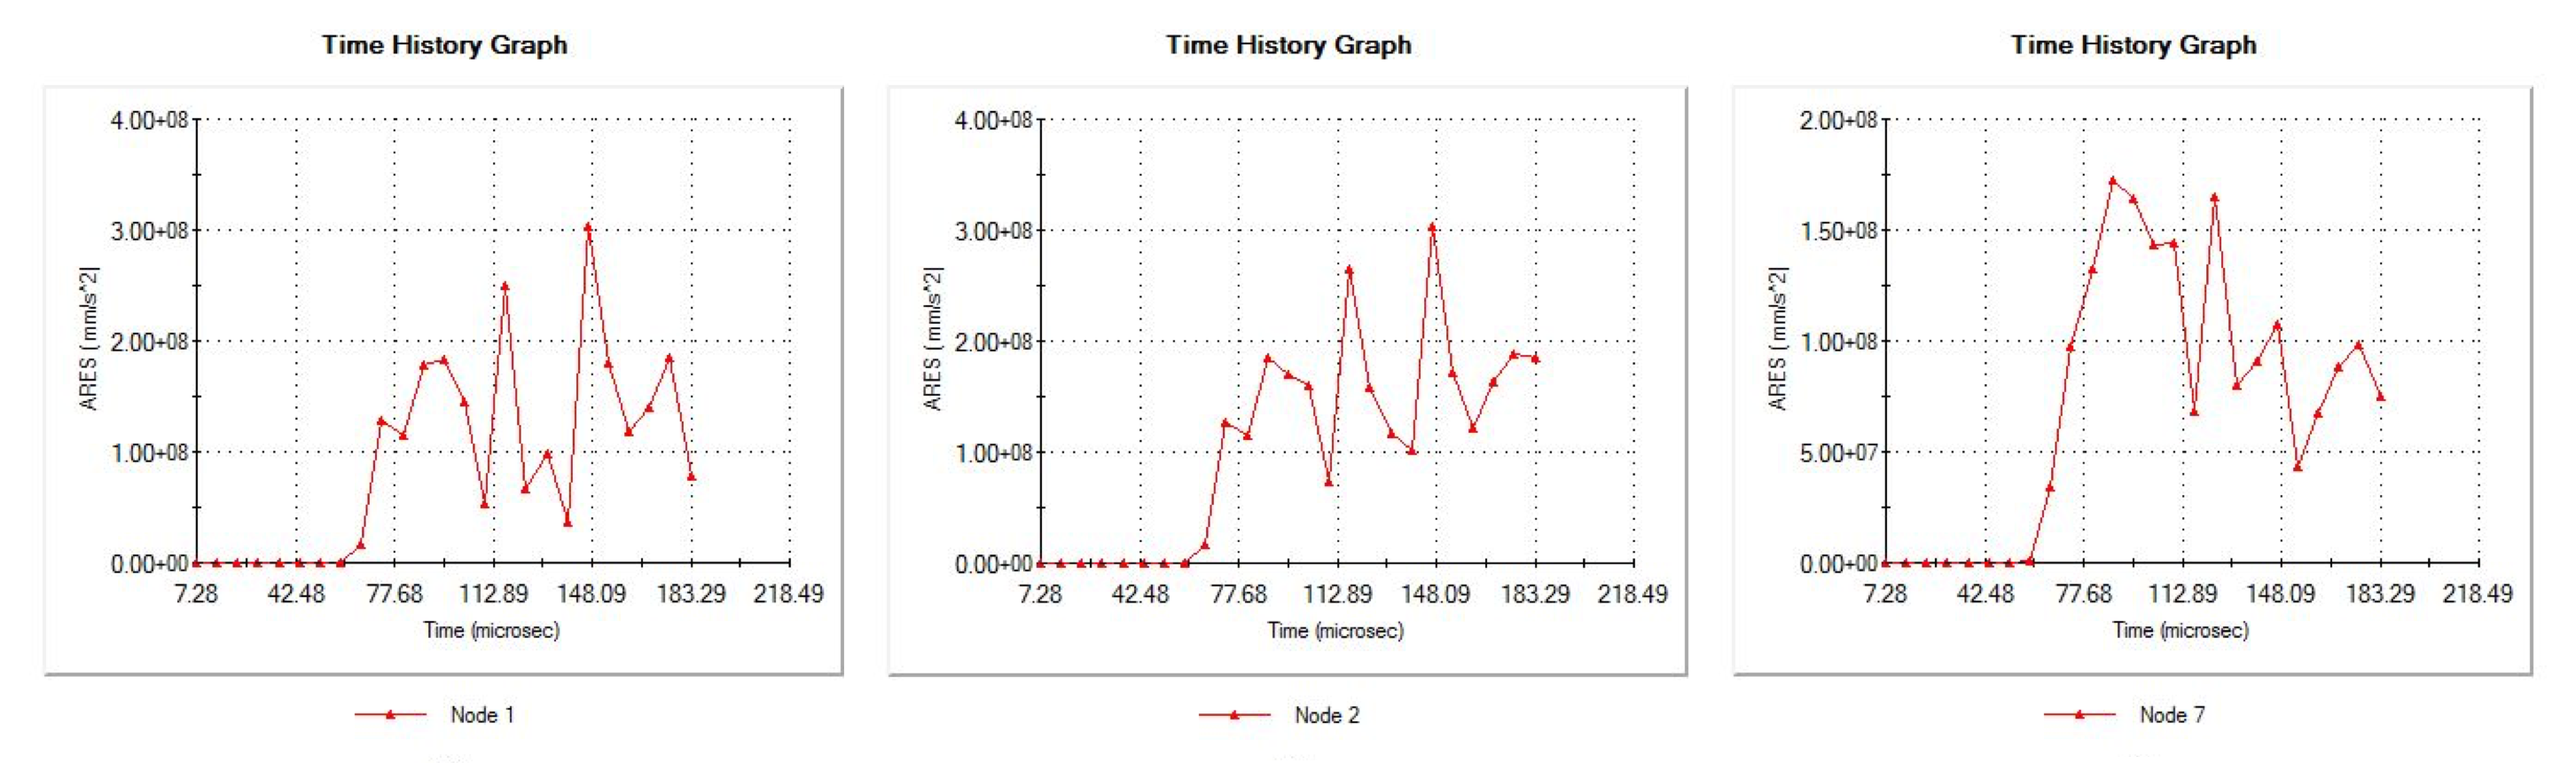
\includegraphics[width=1.95\columnwidth]{figures/db_dt3_res}
  \caption{response graphs for Drop Test 3 for double bone in three different location (nodes).}
    ~\label{fig:db_dt3_res}
\end{figure*}

\subsection{2017/04/18: Frequency Propagation of double bone model}

After discussion, we decided to expand the analysis into a design where the vibration signal of a certain frequency is provided at one end of the bone. This is to simulate a proposed engineering design that the user put his or her arm onto the surface of a smart phone which generates a certain frequency, then another smart phone, held in the hand of the arm, records the propagated frequencies with accelerators to determine the bone density.

Therefore, instead of the original design where only one impulse is provided, a constant vibration of a certain frequency is provided. There are no obvious built-in SolidWorks package to facilitate this design, but I found "Linear Dynamic Simulation", which uses frequencies and mode shapes to study linear response to dynamic loading, promising for our analysis.

\subsubsection{Linear dynamic modeling of frequency propagation} 

Earlier, I was trying to perform linear dynamic modeling would be a very interesting simulation because it can take into account the impact of a ball towards the bone, which can support an existing measurement equipment in the lab. Unfortunately, when I was running the simulations, the SolidWorks crashed several times and never made to the end. I will re-attempt this simulation. The following is to simulate the frequency propagation.

I attempted to create a harmonic dynamic simulation. In doing so, one essential step is to create a periodic force as the constant impulse and record the time steps of the propagation. Searching for different resources, I found it currently infeasible for such task. Consulting several friends in mechanical engineering and material sciences, they suggest that SolidWorks was mostly used for model design and ANSYS is the common software for simulations, so I decide to switch gear to ANSYS.

\subsubsection{FEA with ANSYS} 

ANSYS is only available through ME departmental access in the remote desk top. To specify material properties of the bone, there is only one built-in material available in their package, thus, when specifying a new type of material, I defined the density to be 1900 $kg/m^3$ from \cite{Cameron:1999:Physics}. So far, the ANSYS simulation has not been fully finished yet. 

However, in the midst, some of my friends in mechanical engineering let me know that such simulation, even done by ANSYS, will be very difficult if possible as all. Normally, they would just use a vibrator and experiment on the material itself through manual frequency tuning instead of simulation. 

\subsubsection{Cogitation about the propagation process} 

Let's take a step back and think of the process, as shown in equation \eqref{eq:mot1}\eqref{eq:mot2}, an external frequency input would not observe a change in frequency when propagation. The propagation created a phase change and uneven amplitude due to resonance of the material. 

How to define the density of a material, in our case, the bone, is more or less related to the natural frequency of the material. In our experimental design, the way to experimentally determine the frequency is to exert an external frequency changing within a wide range and find the biggest amplitude recorded, which would be the natural frequency which causes resonance.  

\subsubsection{Initial formulation of the frequency analysis} 

Mechanical impedance is a measure of how much a structure resists motion when subjected to a harmonic force. The motion function can be formulated as:

\begin{equation} \label{eq:mot1}
mx''+cx'+kx=f(t)={\bf F}e^{jwt}
\end{equation}

where $f(t)$ is the external force with a harmonic oscillation. Thus, the corresponding harmonic oscillation induced by the external force: 

\begin{equation} \label{eq:mot2}
x={\bf X}e^{j\omega t}, x'={\bf V}e^{j \omega t}=j\omega{\bf X}e^{j\omega t}, x''={\bf A}e^{j \omega t}=-\omega^2{\bf X}e^{j \omega t}
\end{equation}

From many aspect, our question is very similar to the classic beam question. There are several predefined properties discovered in the beam studies which could offer insights into our analysis. If we consider the bone as a beam, for example, a cantilever beam (because one end is attached to the smart phone as a fixed point), then its natural frequency can be expressed by the following \cite{Young:2002:formula}:

\begin{equation} \label{eq:beam}
f_1=\frac{\alpha_1^2}{L^2}\sqrt[]{\frac{EI}{w}}=\frac{\alpha_1^2}{L^2}\sqrt[]{\frac{EI}{\rho A}} 
\end{equation}

where $f_1$ is the natural frequency of the cantilever beam (bone) with uniform load $w$ per unit length including beam (bone) weight; $L$ is the length of the beam (bone); $E$ is the modulus of elasticity of the material; $I$ is the area moment of inertia, a geometrical parameter based on the intersection of the beam (bone); and normally, we take constant $\alpha_1 = 1.875$.

What is interesting in this formula is how bone structure can be specified differently here. The area of inertia can be different as the structural properties of the bone is a porous complex. I can try treating each individual pore as one unit and sum them up together. In addition, the elasticity of the bone is relatively undefined. Other than calculation, another more direct way would be to do an elasticity measurement of a real bone. 
 
The real application in OsteoApp would have more to consider. Not only in our formula it displays that length of arm is a factor to determine natural frequency (something to be collected during user experiments). Moreover, with the addition of muscle, it would be two separate materials instead of one. In that analysis, we need to calculate two natural frequencies separately and combine their amplitudes together to be our estimated signal during measurements. 

\section{Acknowledgments}

Thank Prof. Shwetak Patel for the opportunity to join this exciting lab and work on this meaningful project. Thank Morelle and Josh for the patient guidance and faith in me through the project. Thank UbiComp Lab members for helpful advice and support. Thank Hongtao Wu, Yuxin Fu, Che Yi, and Ziwen Guo for helpful discussion in mechanical engineering and material science. Thank University of Washington for the wonderful platforms and resources in electrical engineering, mechanical engineering and computer science. 

\balance{}


% REFERENCES FORMAT
% References must be the same font size as other body text.
\bibliographystyle{SIGCHI-Reference-Format}
\bibliography{sample}

\end{document}

%%% Local Variables:
%%% mode: latex
%%% TeX-master: t
%%% End:
